\chapter{相关开发技术与环境}
\section{SpringBoot框架}
\subsection{SpringBoot框架核心理念}
在Java企业级应用的演化进程中，以Spring、Spring MVC及MyBatis为代表的传统架构曾占据主导地位。然而，这类架构在实际工程落地时，往往伴随着繁杂的XML文件配置、冗长的依赖版本管理以及多步骤的部署流程。开发人员在启动新项目时，必须耗费大量精力去处理各类框架间的整合与组件装配，无形中降低了生产效率。为打破这一应用僵局，Spring Boot框架应运而生。

作为Spring生态体系的深度扩展，Spring Boot的设计初衷是实现“开箱即用”。其最核心的指导原则在于“约定优于配置”。该机制通过提供科学的默认参数，极大地削减了传统开发模式下的样板代码与配置文件。在日常开发中，无需进行繁琐的底层结构搭建，仅需通过少量的注解指令即可接管Bean的管理与自动化装配。这种轻量化的框架重构，不仅使得Web应用的搭建更加灵活，也让开发者的精力得以从底层环境部署中抽离，重新聚焦于核心业务逻辑的实现。
\subsection{SpringBoot框架关键特性}
在现代软件工程中，Spring Boot之所以能够逐渐取代老旧的开发模式，主要得益于其独具优势的几大核心技术特性：
\begin{enumerate}[label=(\arabic*)]
	\item \textbf{解耦机制：}
	继承自Spring生态的底层精髓，Spring Boot深度践行了控制反转（IoC）理念。对象组件的创建与生命周期管理不再由开发者在代码中硬性实例化，而是全权交由框架的IoC容器统一调配。借助依赖注入（DI）技术，系统在运行期间能够通过简单的注解，将关联的实例动态注入到目标对象中。这种机制从根本上剥离了业务模块间的强耦合关系，极大地提升了系统的可测试性与扩展性。
	\item \textbf{起步依赖：}
	框架提供了一种高度聚合的构建与依赖管理方案。结合Maven等项目构建工具，Spring Boot将特定功能场景（如Web通信、安全框架等）所需的庞杂底层类库，封装为标准化的“起步依赖”。当开发者在项目的pom.xml文件中引入某一Starter时，其核心依赖管理机制能够自动下载所需库文件并处理传递性依赖，彻底解决了以往手动排查Jar包冲突的繁琐问题，显著提升开发效率。
	\item \textbf{外部化配置：}
	在企业级软件生命周期的演进过程中，系统往往需要经历本地开发、集成测试与正式生产等多个阶段。面对不同环境下各异的数据库网关、中间件端口及第三方服务密钥等差异化参数，Spring Boot 提供了极具弹性的外部化配置机制。开发团队可以为特定的运行环境预设独立的分支配置文件（如 application-dev.yml 与 application-prod.yml）。在项目构建打包后，运维人员无需对系统源码进行任何重新编译或修改，仅需在服务启动时通过命令行参数、系统环境变量或注册中心，动态声明当前激活的配置集，即可完成复杂环境的无缝切换。这种设计模式，彻底实现了核心业务代码与物理环境参数的深度解耦，极大地提升了项目的交付效率与工程化管理水平。
	\item \textbf{内嵌式运行容器：}
	传统Java Web项目通常需要打包为War格式，并强依赖于外部配置好的Tomcat服务器进行部署。Spring Boot则打破了这一常规，其内部直接集成了主流的Web容器环境。通过打包指令，整个项目及其运行环境可被封装为一个独立的可执行Jar包。只需极简单的终端命令行交互即可直接启动服务，这不仅简化了运维层面的操作步骤，更使其成为现代微服务架构体系下的首选基础框架。
	% 表格与下文之间空一行
\end{enumerate}

\section{Vue框架}
在现代前端工程化实践中，Vue.js 凭借其轻量级与“渐进式”（Progressive）的设计理念，已成为构建交互式用户界面的主流方案之一。所谓渐进式，即该框架允许开发者根据项目复杂度，从简单的页面局部视图增强，平滑过渡到基于全家桶构建复杂的单页应用（SPA）。与传统强依赖频繁操作真实 DOM 节点的库（如 jQuery）不同，Vue2 框架在底层深度贯彻了 MVVM（Model-View-ViewModel）架构模式，如图\ref{fig:mvvm-pattern-diagram}所示。
\begin{figure}[htbp]
	\centering
	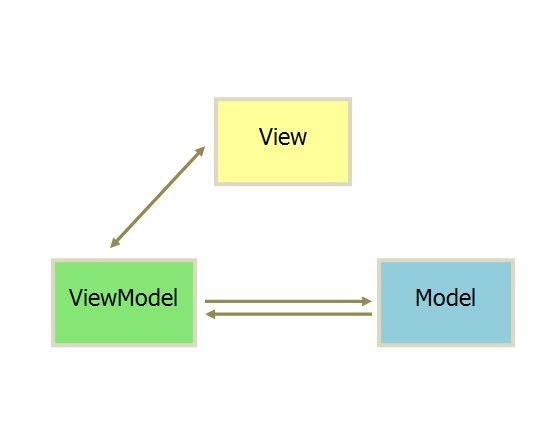
\includegraphics[width=0.68\linewidth]{imgs/MVVM模式图.jpg}
	\caption{MVVM模式图}
	\label{fig:mvvm-pattern-diagram}
\end{figure}

在该架构中，Model 层负责业务逻辑与数据状态的存储；View 层代表视觉呈现界面；而 ViewModel 层则是 Vue 框架的核心枢纽。ViewModel 通过数据绑定技术将数据模型与视图结构桥接起来，当模型数据发生变更时，视图会自动进行同步更新；反之，当用户与视图产生交互时，数据的状态也会被即时捕获。这种双向通信机制彻底剥离了繁琐的底层节点操作，使得前端工程的重心得以回归到核心业务数据的流转上。

主流的前端框架除了Vue，还有React和Angular。对比于 React 框架，Vue 在视图渲染效能、语法直观性及周边生态储备上表现出显著的优越性。在页面重绘机制上，Vue 依托精细的响应式追踪机制配合虚拟 DOM 与 Diff 算法，能够以极高的精度定位视图层中需变更的最小范围，从而大幅削减不必要的渲染开销。就编码体验而言，其高度提炼的模板语法极大地降低了代码的晦涩感，提升了业务模块的开发速率。同时，其背后沉淀的庞大开源社区与海量高质量插件，为复杂功能的快速落地提供了坚实的扩展支撑。
另一方面，相较于体量庞大的 Angular ，Vue 有着轻量化的架构设计、平缓的学习曲线以及高内聚的模块化管理。它摒弃了冗余的默认规范约束，赋予了项目极高的配置自由度，使工程脚手架的搭建能够精准贴合实际业务诉求。其出色的架构弹性不仅允许作为独立库无缝嵌入传统项目，还能在组件化模式下保持数据流转的清晰透明，极大便利了后期的代码审阅与缺陷排查。

结合本系统对开发周期、代码可维护性以及复杂表单交互效率的工程要求，Vue 框架具备轻量灵活、学习成本低、生态完善等优势，因此选择 Vue 来搭建系统的前端。

\section{数据库技术}
在企业级 Web 应用的系统架构中，数据持久化与高并发读写性能是衡量系统健壮性的核心指标。为了兼顾数据的强一致性约束与系统的高频访问响应速度，本系统在数据存储层采用了MySQL来进行数据的持久化，利用Redis的高性能来降低接口响应时间。
\subsection{关系型数据库MySQL}
MySQL 是目前全球应用最为广泛的开源关系型数据库管理系统之一，它的基础架构基于C++实现，因此有着卓越的查询性能。MySQL官网支持主流的操作系统，有着极低的部署成本以及庞大的开发者生态。其运行机制如图\ref{fig:sql-execution-diagram}所示。
\begin{figure}[htbp]
	\centering
	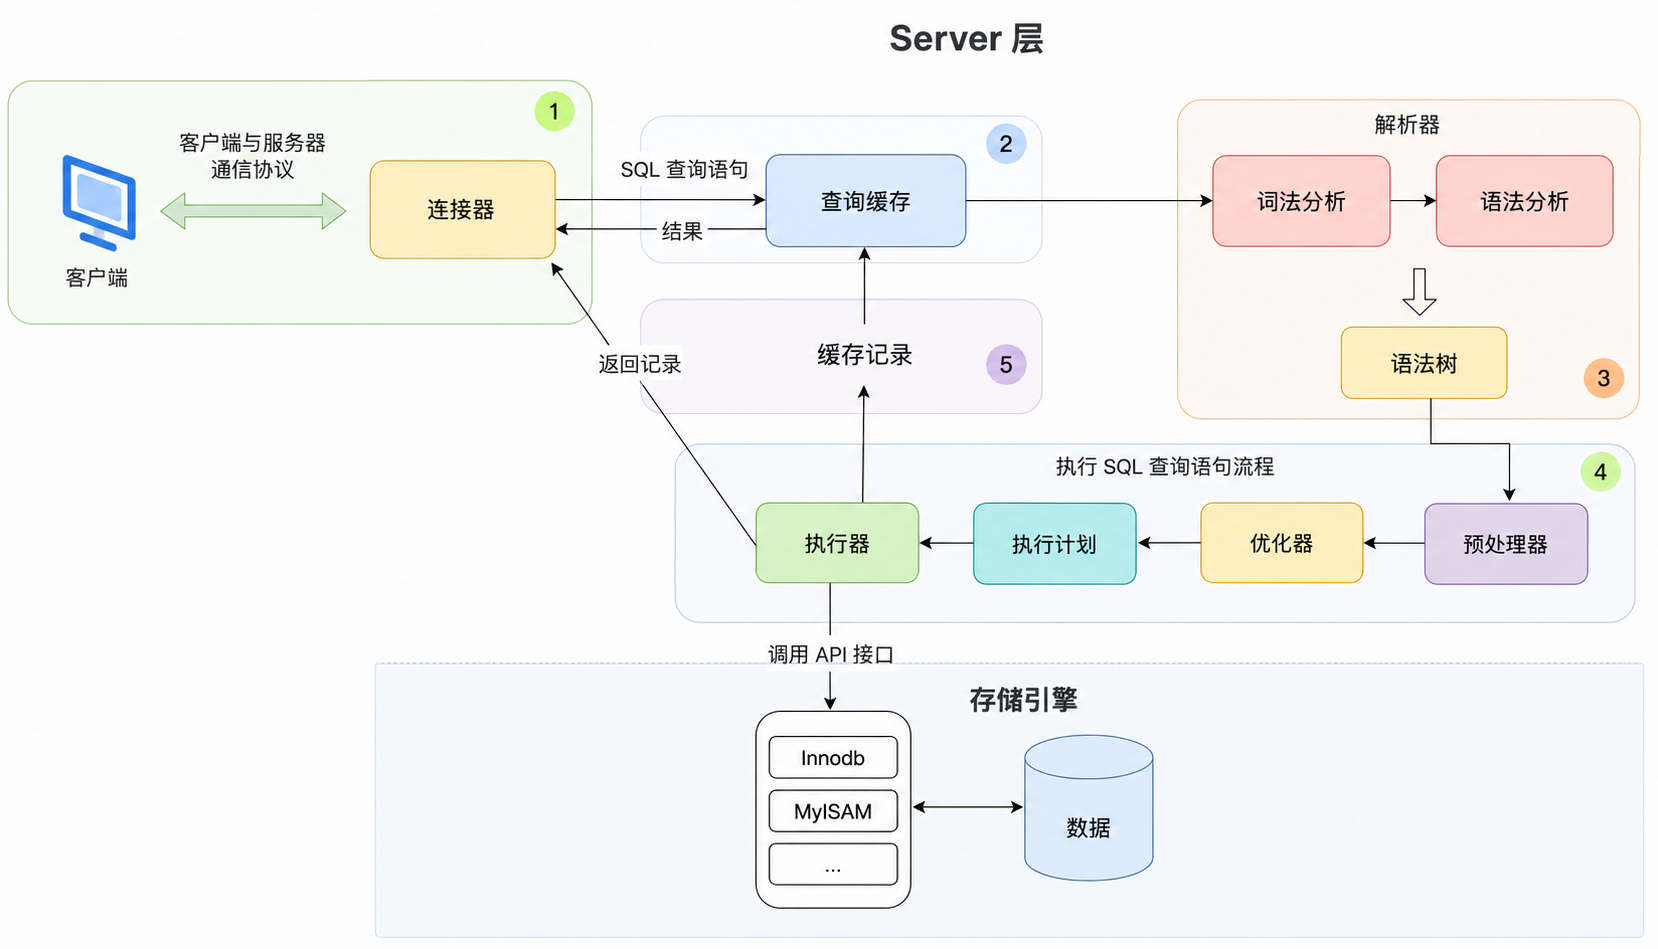
\includegraphics[width=0.68\linewidth]{imgs/SQL执行过程.png}
	\caption{MySQL执行流程图}
	\label{fig:sql-execution-diagram}
\end{figure}

客户端通过TCP协议连上 MySQL 服务后，会先做权限校验和身份确认，这一步由连接器负责，为了提高速度和资源利用率，MySQL会用连接池来进行连接。接着，系统会看看之前有没有执行过一模一样的 SQL（但是查询缓存在最新的MySQL版本中因为命中率太低被移除了）。之后这条查询语句会走到解析器那里，做词法和语法检查，看看语句写得对不对；然后再交给预处理器，验证里面涉及的表和字段是不是真的存在。再往后就是优化器登场，它会根据各种情况算一算哪种执行方案成本最低，比如决定用哪个索引来查。最后执行器按这个计划去调用存储引擎提供的接口，把符合条件的记录一条条取出来，最终将结果集打包返回给客户端。

本系统选用其默认的 InnoDB 存储引擎，该引擎不仅提供了对 ACID（原子性、一致性、隔离性、持久性）事务的完整支持，底层更依托 B+ 树数据结构构建索引，极大地优化了数据检索的磁盘 I/O 效率。同时，InnoDB 通过引入 MVCC（多版本并发控制）机制与行级锁，有效解决了高并发场景下的读写冲突，保障了多线程环境下的数据隔离与一致性。
\subsection{非关系型数据库Redis}
虽然 MySQL 能够提供稳定可靠的数据持久化服务，但在面对海量并发访问或热点数据高频查询等低延迟交互场景时，传统关系型数据库易面临严重的磁盘 I/O 瓶颈，为此，本系统引入了 Redis 作为非关系型数据库。Redis 本质上是一款由c语言实现的，基于内存的高性能键值对存储系统，由于其数据读写操作主要在 RAM 中进行，能够实现亚毫秒级的响应延迟与极高的吞吐量。除了基础的字符串类型，Redis 还原生支持哈希、列表、集合、有序集合等丰富的数据类型，开发者能够很便捷地将其应用于排行榜，分布式锁，打卡签到等场景。为了兼顾数据安全性，Redis提供了RDB快照和AOF日志两种持久化方式，前者定期保存全量数据，后者以追加形式记录每条写命令，两者可组合使用或采用混合持久化以平衡恢复速度与数据完整性。在性能方面，Redis采用单线程模型处理命令，避免了多线程的锁竞争和上下文切换开销，同时借助I/O多路复用技术让单个主线程能够并发处理大量客户端连接。基于以上特性，在流量较大或者数据库查询比较慢的接口，引入 Redis 可以有效减少到达数据库的请求数量，提高系统的性能和稳定性。

\section{Echarts库}
ECharts是一款基于JavaScript编程语言实现的开源Web数据可视化库，常用于在网页中呈现各类统计图表。该库支持折线图、柱状图、饼图、散点图以及地图等多种常见图表类型，并且允许在同一图表中组合多种图形。开发时只需通过一个配置对象指定图表的样式与数据，ECharts便会自动完成渲染，并内置了缩放、悬停提示等交互功能。底层可选用Canvas或SVG两种渲染方式，能够适应从少量数据到大规模数据的展示需求。在本系统的前端模块中，使用ECharts将后台统计数据以直观的图表形式呈现，便于用户快速获取信息。

\section{MyBatis-Plus}
MyBatis-Plus是一个基于Java编程语言实现的持久层框架，它在MyBatis的基础上提供了一层轻量级的封装，核心设计理念是“只做增强不做改变”，即完全兼容原生MyBatis的所有特性，同时通过内置通用Mapper、条件构造器和代码生成器等组件大幅简化数据库访问层的开发工作。在实际使用中，持久层接口只需继承MyBatis-Plus提供的BaseMapper接口，即可自动获得单表增删改查的全部方法，无需为每个表手动编写相应的SQL语句和映射配置。对于查询条件较为复杂的场景，MyBatis-Plus提供了灵活的Wrapper条件构造器，支持通过Lambda表达式以编程方式动态拼接WHERE条件，不仅规避了XML配置文件中SQL语句的编写工作，还通过方法引用的形式避免了字段名拼写错误等潜在问题。在批量数据处理和分页查询方面，该框架内置了分页插件，能够在数据库层面实现物理分页，开发者只需传入页码和每页条数即可完成分页查询，无需关心底层不同数据库的分页语法差异。对于多表关联查询等复杂场景，MyBatis-Plus保留了手写SQL的能力，开发者仍可在XML或注解中编写原生MyBatis语句，与框架提供的通用CRUD操作共存互补，兼顾了开发效率与底层控制的灵活性，使得开发者能够将更多精力聚焦于业务逻辑，在Java后端项目中被广泛采用。

\section{本章小结}
本章围绕系统开发所依赖的关键技术进行了概述。后端采用SpringBoot框架，借助其自动装配与内嵌容器机制简化服务端开发与部署流程；前端选用Vue框架，介绍了MVVM模式实现视图与数据的双向绑定，降低前端交互的开发复杂度。数据层采用MySQL与Redis组合方案，前者用来管理系统持久化到磁盘的数据，后者通过内存缓存加快响应速度。MyBatis-Plus简化了持久层的CRUD编码，ECharts为数据可视化提供了图表支撑。